\section*{Método de análisis de datos}
\addcontentsline{toc}{section}{Método de análisis de datos}

El análisis de datos se realizará mediante un flujo de ciencia de datos orientado
a series temporales. Primero se depurarán los registros, eliminando duplicados,
tratando valores faltantes y verificando consistencia en fechas, precios y
volúmenes. Luego se construirán variables temporales como mes, semana, temporada
y rezagos del precio FOB, además de variables derivadas para rentabilidad.

Para la evaluación predictiva se utilizarán las siguientes métricas:

\begin{itemize}
  \item \textbf{MAE:} mide el error absoluto promedio del pronóstico.
  \item \textbf{RMSE:} penaliza con mayor fuerza errores grandes.
  \item \textbf{MAPE:} expresa el error porcentual y facilita la interpretación
  para usuarios no técnicos.
\end{itemize}

Los modelos se compararán sobre el mismo conjunto de prueba temporal. El modelo
seleccionado será aquel que logre el mejor equilibrio entre precisión,
estabilidad e interpretabilidad para el productor. Además, los resultados se
integrarán con escenarios económicos para estimar margen y ganancia esperada por
campaña.

\subsection*{Flujograma para seleccionar la prueba estadística}
\addcontentsline{toc}{subsection}{Flujograma para seleccionar la prueba estadística}

Para la contrastación de hipótesis se partirá siempre de estadística
descriptiva, reportando medidas de tendencia central, dispersión y distribución
de los datos. Luego se seleccionará la prueba inferencial según el diseño del
estudio, el número de mediciones, la escala de las variables y el supuesto de
normalidad. La normalidad se verificará con Shapiro-Wilk cuando $n \leq 50$ y
con Kolmogorov-Smirnov cuando $n > 50$.

\begin{figure}[H]
\caption{Flujograma para seleccionar la prueba estadística en la contrastación de hipótesis}
\centering
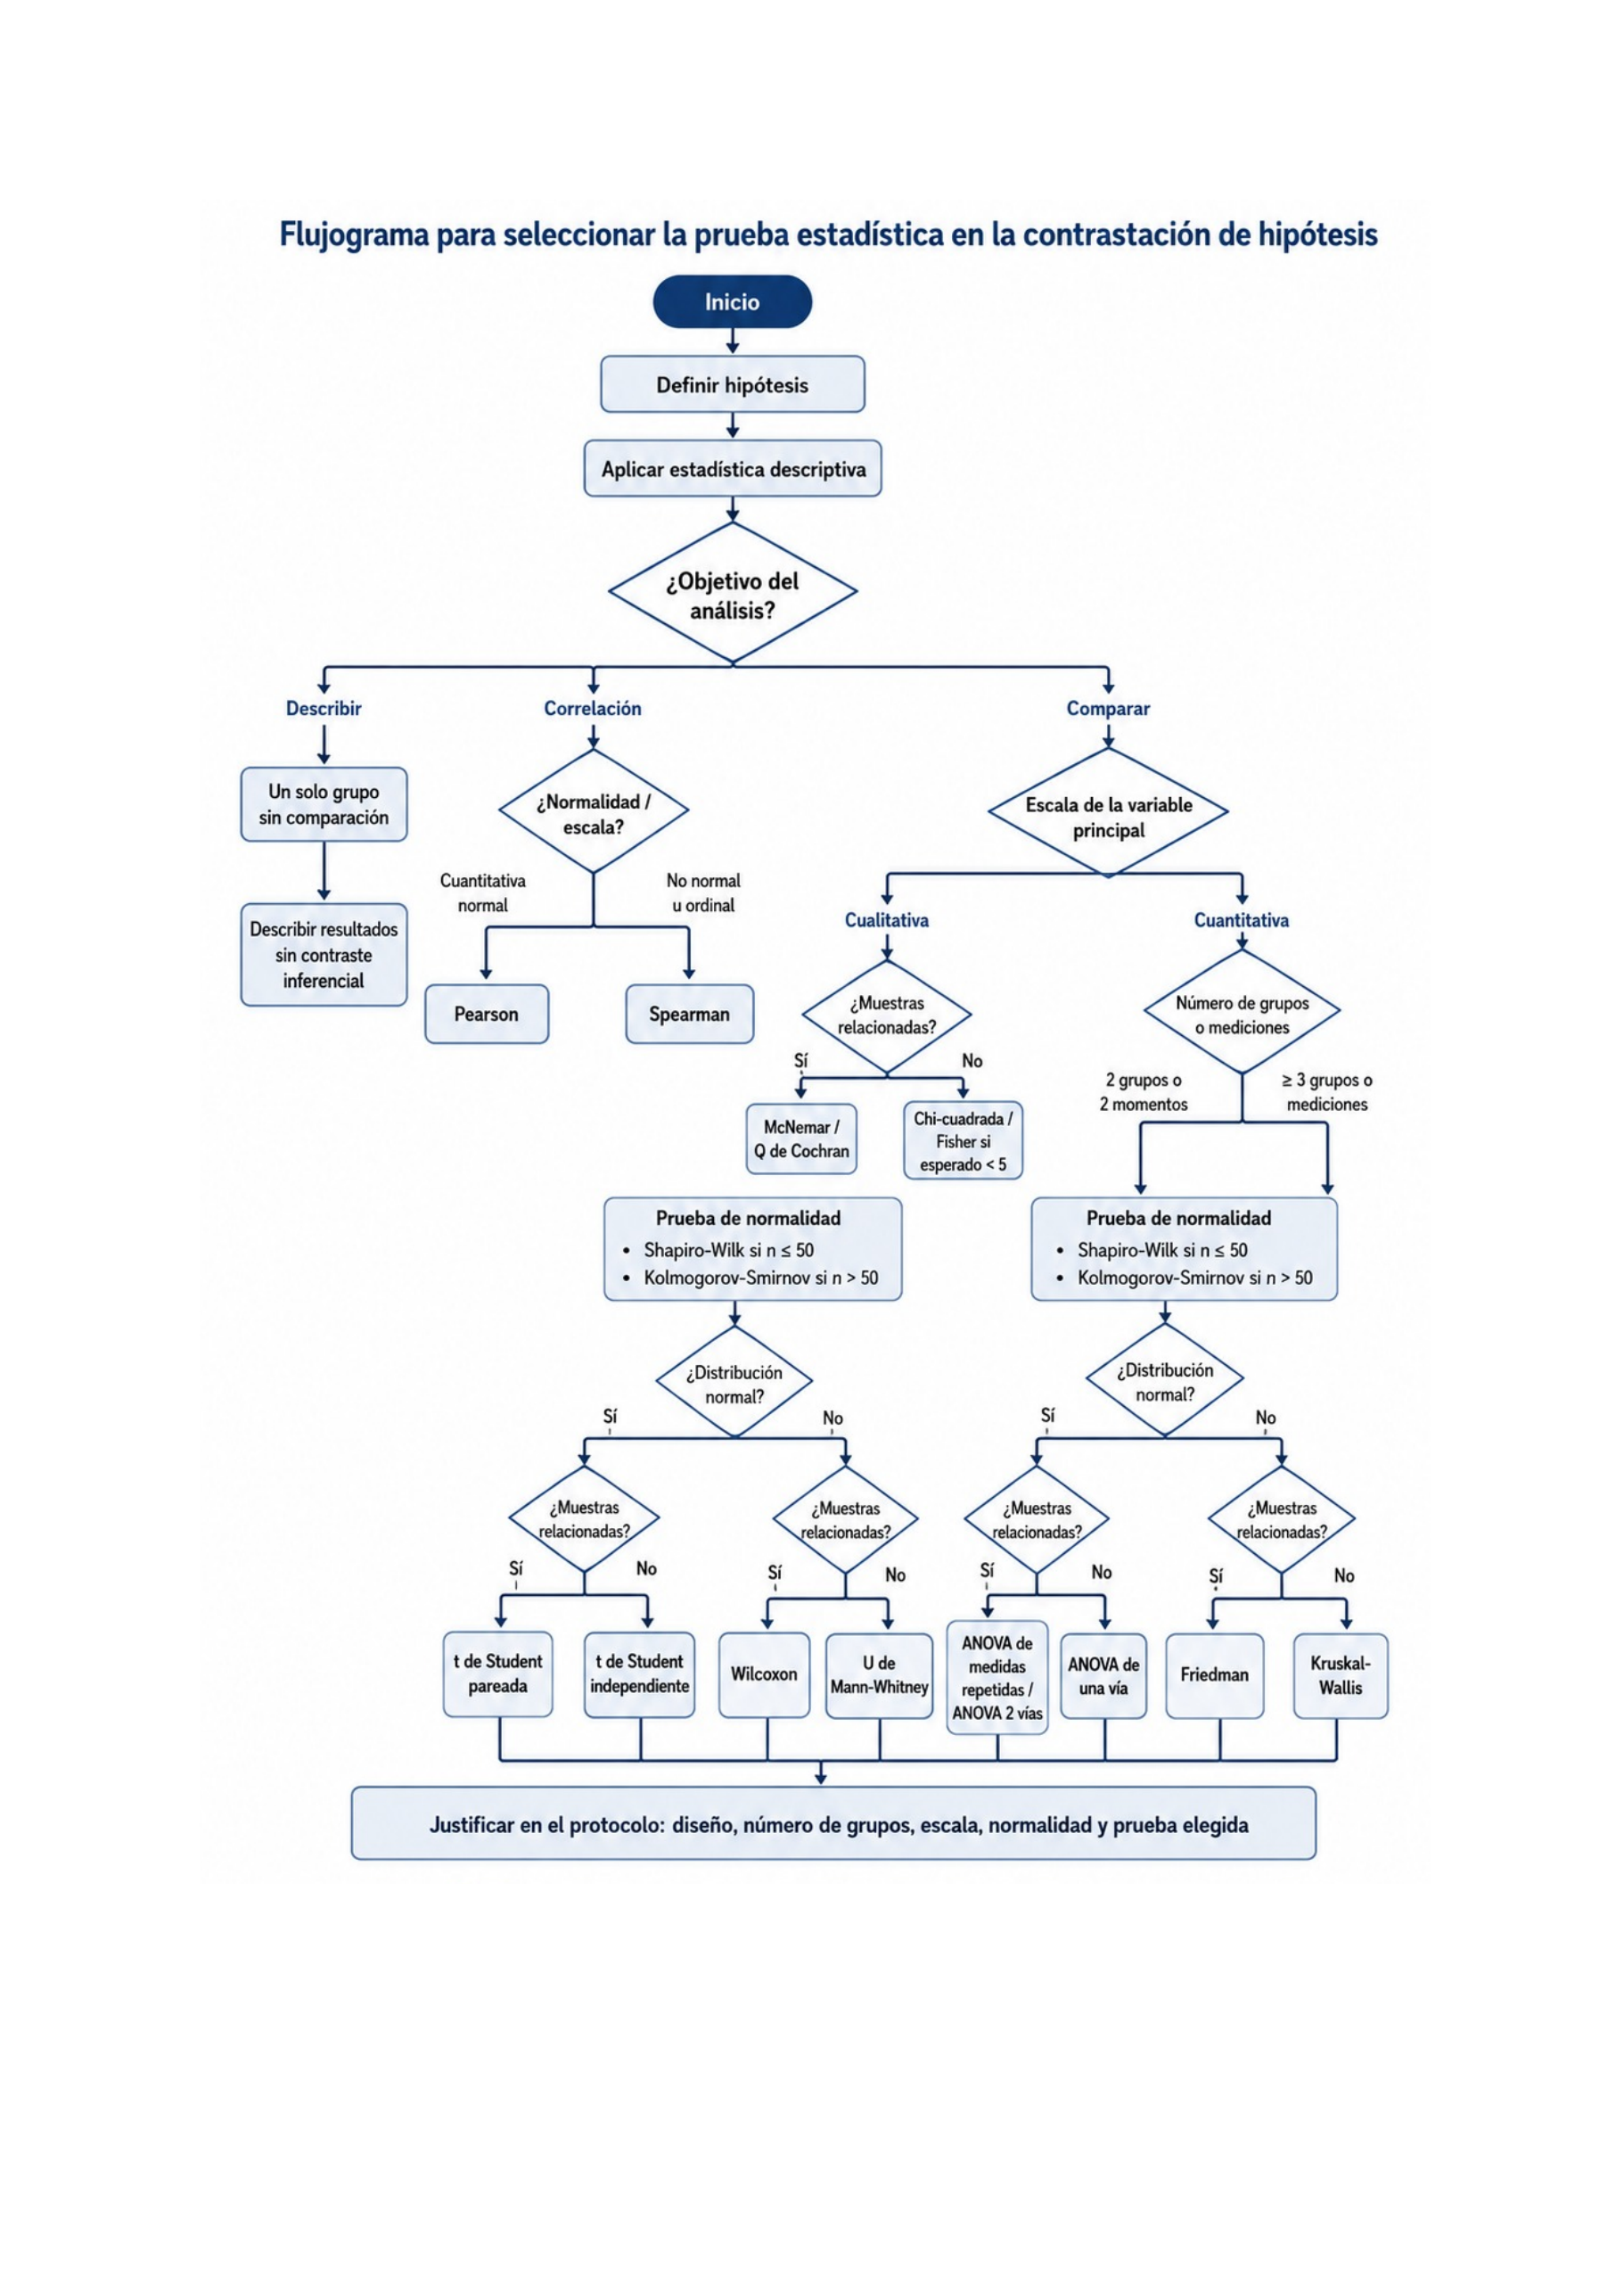
\includegraphics[width=\textwidth]{assets/images/chapter-02/flujograma_prueba_estadistica.png}
\end{figure}

La elección de la prueba deberá justificarse en el protocolo indicando: Diseño
del estudio, número de grupos o mediciones, escala de la variable, resultado de
la prueba de normalidad y criterio aplicado para seleccionar la prueba final.

\subsection*{Contrastación de hipótesis}
\addcontentsline{toc}{subsection}{Contrastación de hipótesis}

La contrastación de hipótesis seguirá el criterio metodológico presentado en la Figura 2.1. En primer lugar, se realizará estadística descriptiva para resumir las variables de estudio. En segundo lugar, se verificará la normalidad de los datos mediante Shapiro-Wilk cuando el tamaño muestral sea menor o igual a 50, y mediante Kolmogorov-Smirnov cuando sea mayor a 50. En tercer lugar, se seleccionará la prueba inferencial paramétrica o no paramétrica según la escala de medición, el número de grupos o mediciones y la relación entre muestras.

El nivel de significancia será $\alpha = 0.05$. La hipótesis nula se rechazará cuando el valor $p$ sea menor que 0.05. En caso contrario, no se contará con evidencia estadística suficiente para rechazarla.

\begingroup
\scriptsize
\setlength{\tabcolsep}{2pt}
\begin{longtable}{p{0.9cm}p{3.5cm}p{5.1cm}p{3.4cm}}
\caption{Pruebas estadísticas para la contrastación de hipótesis específicas}\\
\toprule
\textbf{Hip.} & \textbf{Variables a contrastar} & \textbf{Normalidad y prueba seleccionada} & \textbf{Criterio de rechazo} \\
\midrule
\endfirsthead
\toprule
\textbf{Hip.} & \textbf{Variables a contrastar} & \textbf{Normalidad y prueba seleccionada} & \textbf{Criterio de rechazo} \\
\midrule
\endhead
He1 & Estimación de rentabilidad antes y después del módulo de rentabilidad. & Kolmogorov-Smirnov ($n>50$). t de Student relacionada si existe normalidad; Wilcoxon si no existe normalidad. Estadístico: $t$ o $Z$. & Rechazar $H_0$ si $p<0.05$. \\
\midrule
He2 & Nivel de incertidumbre percibida antes y después del simulador de escenarios. & Kolmogorov-Smirnov ($n>50$). t de Student relacionada si existe normalidad; Wilcoxon si no existe normalidad. Estadístico: $t$ o $Z$. & Rechazar $H_0$ si $p<0.05$. \\
\midrule
He3 & Errores RMSE y MAPE de SARIMA frente a LSTM en el conjunto de prueba. & Shapiro-Wilk si se comparan errores mensuales de prueba ($n\leq50$). t de Student pareada si existe normalidad; Wilcoxon si no existe normalidad. Estadístico: $t$ o $Z$. & Rechazar $H_0$ si $p<0.05$ y el modelo propuesto presenta menor error. \\
\midrule
He4 & Nivel de identificación de patrones antes y después del análisis histórico interactivo. & Kolmogorov-Smirnov ($n>50$). t de Student relacionada si existe normalidad; Wilcoxon si no existe normalidad. Estadístico: $t$ o $Z$. & Rechazar $H_0$ si $p<0.05$. \\
\midrule
He5 & Nivel de interpretación antes y después de utilizar reportes de ciclos. & Kolmogorov-Smirnov ($n>50$). t de Student relacionada si existe normalidad; Wilcoxon si no existe normalidad. Estadístico: $t$ o $Z$. & Rechazar $H_0$ si $p<0.05$. \\
\bottomrule
\end{longtable}
\endgroup

Para las hipótesis vinculadas con productores, la hipótesis nula general indica que no existen diferencias estadísticamente significativas entre las mediciones antes y después de aplicar la solución propuesta. La hipótesis alterna sostiene que sí existen diferencias estadísticamente significativas. Para la comparación SARIMA-LSTM, la hipótesis nula indica que no existen diferencias significativas entre los errores de ambos modelos, mientras que la hipótesis alterna establece que uno de los modelos presenta mejor desempeño predictivo según RMSE y MAPE.

\subsection*{Síntesis de la metodología estadística}
\addcontentsline{toc}{subsection}{Síntesis de la metodología estadística}

El análisis inferencial se aplicará en la sección de resultados con el propósito de validar si las soluciones propuestas generan mejoras estadísticamente significativas. Para el modelo predictivo se compararán los errores de SARIMA y LSTM mediante RMSE y MAPE. Para los módulos orientados al productor se aplicarán mediciones antes y después de usar el sistema, evaluando utilidad percibida, reducción de incertidumbre, mejora en interpretación y estimación de rentabilidad. En todos los casos se reportarán el estadístico de prueba, el valor $p$, el nivel de significancia y la decisión respecto de cada hipótesis.
